\chapter[Estutura Analítica do Projeto]{Estutura Analítica do Projeto}
\addcontentsline{toc}{chapter}{Estutura Analítica do Projeto}

Com o Escopo acertado e alterado desde a primeira sprint até a segunda sprint, foi definida então a EAP (Estrutura Analítica do Projeto) do Grupo 3 da Disciplina “Projeto Integrador de Engenharia 1”, pois trata-se de uma importante ferramenta para o auxílio do gerenciamento do projeto e para o desenvolvimento do cronograma de atividades. Para a confecção da EAP, utilizou-se o software de edição de slides e imagens chamado Microsoft Office Powerpoint.

\begin{figure}[p]
	\centering
    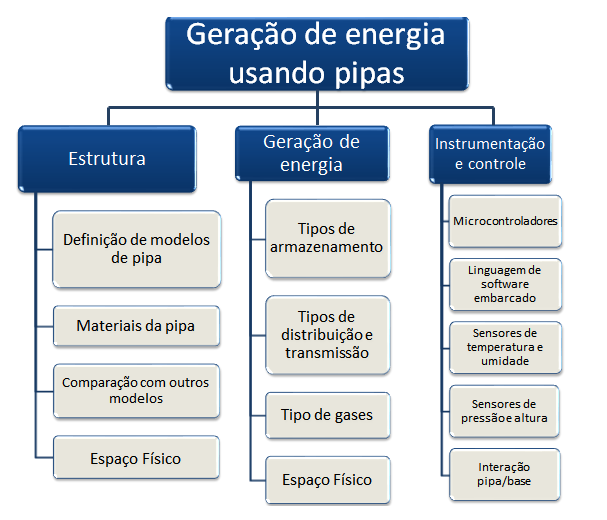
\includegraphics[width=0.8\textwidth]{figuras/eap.png}
    \caption{Estutura Analítica do Projeto}
    \label{fig:eap}
\end{figure} 